% Ajustement, taux d'évolution et tableur, suite géométrique

\section{Dépenses de santé (7 points)}

Le tableau suivant, extrait d'une feuille d'un tableur, donne la consommation de soins et de biens médicaux en milliards d'euros depuis l'année 2000.

\begin{center}
	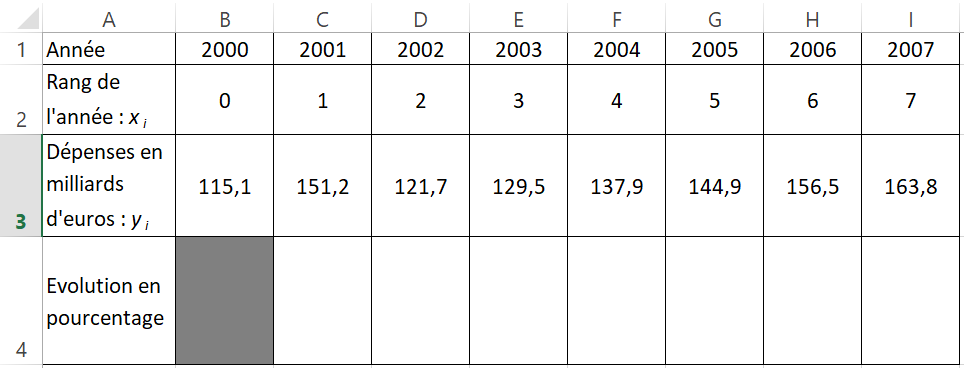
\includegraphics[scale=0.65]{img/biens_medicaux2}
\end{center}

\emph{Il n'est pas demandé de compléter le tableau.}

\subsection{Droite d'ajustement}

\begin{questions}
	\question[1] On suppose que la droite d'ajustement entre le rang de l'année $x$ et les dépenses en milliards d'euros $y$ a pour équation : $y = 7x + 115$. En utilisant cette équation, déterminer le montant des dépenses en 2010. 

\end{questions}

\subsection{Pourcentage d'évolution}

\begin{questions}
	\question[1] Quel est le pourcentage d'évolution global entre 2000 et 2007, à \num{0.1} \% prês ? 

	\question[1] Quelle formule doit-on entrer en $C4$ pour déterminer le taux d'évolution des dépenses entre 2000 et 2001 et pouvoir la recopier vers la droite jusqu'en $I4$ ?
\end{questions}

\subsection{Limitation des dépenses}

Afin de mieux maîtriser les dépenses de santé, le gouvernement souhaitait, à partir de 2008, que les dépenses liées à la consommation de soins et de biens médicaux n'augmentent que de 2 \% par année. On modélise cette évolution par une suite. On désigne par $u_n$ le montant maîtrisé des dépenses pour l'année (2007 + $n$) en milliards d'euros. On a donc $u_0 = \num{163.8}$.

\begin{questions}
	\question[1] Calculer la valeur de $u_1$ (donner la valeur exacte). 
	
	\question[1] Quelle est la nature de la suite $(u_n)$ ? On précisera les éléments caractéristiques de la suite.
	
	\question[1] Exprimer $u_n$ en fonction de $n$.
	
	\question[1] En supposant que cette modélisation reste valable jusqu'en 2015, à combien peut-on estimer le montant des dépenses en 2015 ? (Le résultat est à arrondir à $10^{-3}$).
\end{questions}

  